Including power for the WIB, a fully loaded WIB (one WIB plus four FEMBs) requires
12V and draws up to approximately 4~Amps. Therefore, the full electronics for one APA (one PTC, five WIBs, and 20 FEMBs) 
requires 12V and draws approximately 20A, for a total power of almost 250W, as 
described in Section~\ref{sec:fdsp-tpc-elec-design-warm}.

As the LV power is delivered at 48V to the PTC, each LV power mainframe should 
operate at roughly 30-60V/13.5A/650W maximum capacity. Using 10~AWG cable, an 0.8V drop is expected along the cable with a
required power of 306.12W out of 650W available. 

Four wires will be used for each module, two 10~AWG,
shielded, twisted pair for the power and return, two 20~AWG, shielded, twisted pair for the sense. Sense line fusing will be
provided on the PTC card. This fusing would serve as
a final protection. The primary protection would come from the Over Current protection
on the LV supply modules, which is set above the $\sim$20~Amps. The LV power cable uses FCi micro TCA connectors, 
shown in Figure~\ref{fig:tpcelec-power_conn}.

\begin{dunefigure}
[FCi micro TCA power connector at the PTC end of the cable.]
{fig:tpcelec-power_conn}
{FCi micro TCA power connector at the PTC end of the cable.}
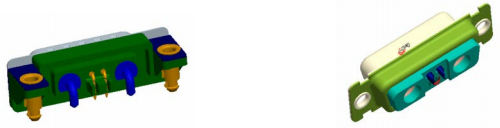
\includegraphics[width=0.9\linewidth]{tpcelec-power_connector.png}
\end{dunefigure}

Each APA requires three wire-bias voltage connections 
at $+$820V, $-$370V, and $-$665V, as described in Section~\ref{sec:fdsp-tpc-elec-design-bias}.
The remaining five wire-bias voltage lines supply between 1 and 1.5~kV to the field cage terminations (3)
and electron diverters (2).
The current on each of these supplies is expected to be zero at normal operation.
However the ripple voltage on the supply must be carefully controlled 
to avoid noise injection into the front-end electronics. Each HV module supplies all the wire-bias power to one APA via
8 SHV connector feedthroughs at the CE flange.

RG-58 coaxial cables connect the wire bias voltages from the mini-crate to the standard SHV
connectors machined directly into the CE feedthrough, so there is no electrical connection between 
the LV power and data connectors and wire-bias voltages. The length of the cables from the Weiner mainframe
to the signal flanges is estimated to be 18~meters.


Optical fibers provide the connections between the WIECs, which act as
Faraday-shielded boxes, to the DAQ and slow control systems.

Duplex LC optical fiber transmits the one GIG-E connection from each
WIB to the slow control system. The WIB reports its onboard temperature and the current draw from each FEMB to the slow control system, while the 
current draw for each APA is monitored at the mainframe itself.
